\documentclass{beamer}
\input{../flat-blue-theme.inc}
\input{../footnotes.inc}

\usepackage[utf8]{inputenc}
\usepackage[OT1]{fontenc}
\usepackage[ngerman]{babel}
\usepackage{lastpage}

\usepackage{tikz}
\usetikzlibrary{
	calc
}

\usepackage[outline]{contour}
\contourlength{1.25pt}

\newcommand{\sarrow}{\small$\rightarrow$}
\newcommand{\tipp}[2][Tipp]{\vspace{0.2cm}\textbf{#1:}\\#2}

\setbeamercovered{invisible}
\beamertemplatenavigationsymbolsempty

\author[Hauke Stieler]{Hauke Stieler\\\href{mailto:4stieler@informatik.uni-hamburg.de}{4stieler@inf}}
\title{Wandern, Trekking \& Co.}
\date{\today}

\begin{document}
	{
		\setbeamertemplate{footline}{}
		\setbeamertemplate{headline}{}
		%		\setbeamertemplate{background}{
\includegraphics[width=\paperwidth,trim=0 0 0 3.5cm]{images/tax-government}}
		\maketitle
		\addtocounter{page}{-1}
	}
	
	\begin{frame}[t]{Inhalt}
	\tableofcontents[hidesubsections]
	\end{frame}
	
	\section{Grundlagen}
		
		\begin{frame}[t]{Inhalt}
			\tableofcontents[currentsection,hideothersubsections]
		\end{frame}
	
		\subsection{Wandern, Trekking, Bushcrafting ... -- Wo ist der Unterschied?}
		
			\begin{frame}{}
				\begin{itemize}
					\item \textbf{Wandern:} Anspruchsvoller Gang durch die Natur.\pause
					\item \textbf{Trekking:} Mehrtägiges Wandern in (meist) entlegeneren und gebirgigen Gebieten.\pause
					\item \textbf{Bushcrafting:} Nur mit grundlegendem Equipment in einer natürlichen Umgebung zurecht kommen.\pause
					\item \textbf{Thru-Hiking:} End-to-end Wanderung eines langen Wanderweges.\pause
					\item \textbf{Ultraleicht Wandern:} Mit wenig und/oder sehr sehr leichtem Gepäck wandern.
				\end{itemize}
			\end{frame}
		
		\subsection{Mythen-Klassiker}
			
			\begin{frame}{}
				\begin{enumerate}
					\item Wandern ist nur was für Outdoor-Freaks / alte Menschen.\pause
					\item Niemals alleine Wandern gehen!\pause
					\item Wandern ist auch nur ein Spatziergang.\pause
					\item Meine wasserdichte GoreTex-Jacke hält mich trocken.\pause
					\item Ohne Merino-Alpaka-Multifunktions-Shirt gehe ich nicht los.\pause
					\item Ohne Profi-Equipment braucht man gar nicht erst los gehen.\pause
					\item Auf längeren Touren muss man Nahrungsergänzungsmittel zu sich nehmen.\pause
					\item Papierkarten? Ich hab doch meine Wander-App.\pause
					\item Wölfe, Bären und Berglöwen wollen mich essen.\pause
					\item Mit einem Erste-Hilfe-Set bin ich sicher.\pause
				\end{enumerate}
			\end{frame}
			
	\section{Equipment \& Navigation}
		
		\begin{frame}[t]{Inhalt}
			\tableofcontents[currentsection,hideothersubsections]
		\end{frame}
		
		\subsection{Equipment}
		
			\begin{frame}{Rucksäcke}
				\begin{itemize}
					\item Maße: Liter (Volumen), Rückenlänge (Passform), Eigengewicht
					\begin{itemize}
						\item Angabe "45+10 L" \textrightarrow\ 45 L Rucksack + 10 L Variabler Anteil
					\end{itemize}\pause
					\item Hüftgurt: Gewichtsverlagerung Schulter \textrightarrow\ Hüfte\pause
					\item Unterschiedliches Design für Frauen \& Männer\pause
					\item Nicht wasserdicht \textrightarrow\ Wasserdichte Regenhülle\pause
					\item Diverse Features: Netz am Rücken, Reißverschlüsse, Außentaschen, Trinksystem, ...
				\end{itemize}
			\end{frame}
			
			\begin{frame}{Rucksäcke: Arten (1/2)}
				\begin{columns}[c]
					\begin{column}{0.64\textwidth}
						\begin{itemize}
							\item \textbf{Tagesrucksäcke}
							\begin{itemize}
								\item Für 0-2 Übernachtungen
								\item Volumen: 5-25 L
								\item Kein oder kleiner Hüftgurt
								\item 30 - 150 €
							\end{itemize}
						\end{itemize}
					\end{column}
					\begin{column}{0.34\textwidth}
						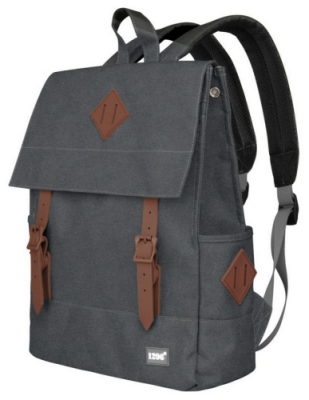
\includegraphics[height=2.25cm]{images/backpack-small.png}
					\end{column}
				\end{columns}
				\vspace{0.4cm}
				\pause
				\begin{columns}[c]
					\begin{column}{0.64\textwidth}
						\begin{itemize}
							\item \textbf{Tourenrucksack}
							\begin{itemize}
								\item Für 1-7 Übernachtungen
								\item Volumen: 25-50 L
								\item Hüftgurt, ggf. Trägersystem
								\item 100 - 300 €
							\end{itemize}
						\end{itemize}
					\end{column}
					\begin{column}{0.34\textwidth}
						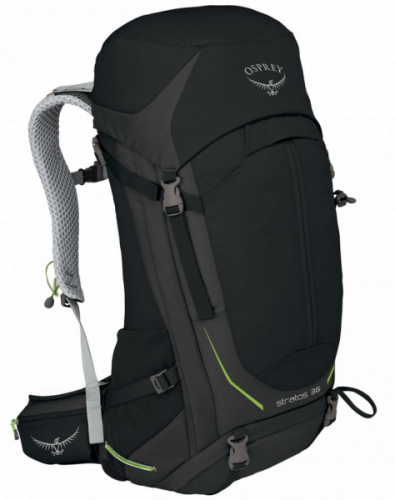
\includegraphics[height=2.5cm]{images/backpack-medium.png}
					\end{column}
				\end{columns}
			\end{frame}
				
			\begin{frame}{Rucksäcke: Arten (2/2)}
				\begin{columns}[T]
					\begin{column}{0.64\textwidth}
						\begin{itemize}
							\item<1-> \textbf{Trekkingrucksack}
							\begin{itemize}
								\item Für 5+ Übernachtungen
								\item Volumen: 45-100 L
								\item Hüftgurt, Trägersystem, ggf. hohes Eigengewicht
								\item 150 - 400 €
							\end{itemize}
							\item<2-> \textbf{Weitere:} Kletterrucksack, Trail-Runner-Rucksack, Skirucksack, ...
						\end{itemize}
					\end{column}
					\begin{column}{0.34\textwidth}
						\onslide<1->{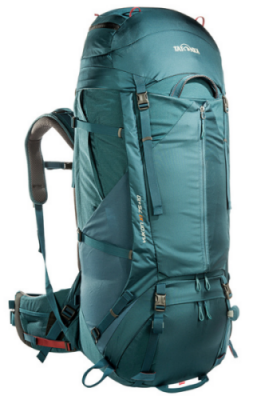
\includegraphics[height=3cm]{images/backpack-big.png}}
					\end{column}
				\end{columns}
			\end{frame}
			
			\begin{frame}{Rucksäcke: Welcher ist der richtige?}
				\begin{itemize}
					\item Was für eine Tour?
					\item Wie viel Equipment?
					\item Wie ist meine Anatomie? \textrightarrow\ Rückenlänge, Hüftbreite, ...
					\item Sind besondere Funktionen nötig/gewünscht?
					\item Tragekomfort \textrightarrow\ Im Laden anprobieren!
				\end{itemize}
			\end{frame}
			
			\begin{frame}{Unterkunft: Zelte \& Tarp}
				\begin{columns}[c]
					\begin{column}{0.69\textwidth}
						\textbf{Zelt:}
						\begin{itemize}
							\item Dach, Wand, Boden + Gestände
							\item Tunnel- / Kuppelzelt
							\item Größe abhängig von Personenanzahl
							\item Sonstige: Autodachzelt, Familienzelt, Strandmuschel, ...
						\end{itemize}
					\end{column}
					\begin{column}{0.29\textwidth}
						\onslide<1->{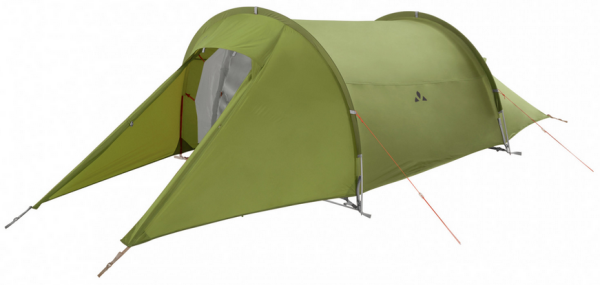
\includegraphics[width=3cm]{images/tent.png}}
					\end{column}
				\end{columns}
				\vspace{0.2cm}
				\pause
				\begin{columns}[c]
					\begin{column}{0.69\textwidth}
						\textbf{Tarp:}
						\begin{itemize}
							\item Zelt ohne Gestänge und Boden
							\item Ggf.: Gestände, Seile, Mückennetz, etc.
							\item Dreieckig, Rechteckig, Fünfeckig, ...
						\end{itemize}
					\end{column}
					\begin{column}{0.29\textwidth}
						\onslide<1->{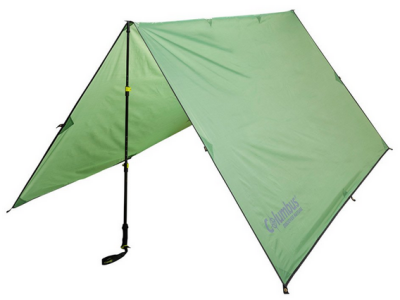
\includegraphics[width=2.5cm]{images/tarp.png}}
					\end{column}
				\end{columns}
			\end{frame}
			
			\begin{frame}{Unterkunft: Zelte \& Tarp -- Vor- \& Nachteile}
				\textbf{Zelt:}
				\begin{itemize}
					\item[$+$] Regen, Wind \& Sichtschutz
					\item[$-$] Schwer: 1,5 - 2,5 kg (1-Personen Zelt)
					\item[$-$] Teuer: 200 - 350 €
				\end{itemize}\pause
				\textbf{Tarp:}
				\begin{itemize}
					\item[$+$] Leicht(er): $<$ 1 kg (manche sogar $<$ 200 g)
					\item[$+$] Billig(er): ab 6,50 € (bis 300 €)
					\item[$-$] Nicht immer geeignet
				\end{itemize}\pause
				\tipp[Tarp Tipp]{Baumarktplane für 6,50 € mit Ösen bei Bauhaus.}
			\end{frame}
			
			\begin{frame}{Unterkunft: Schlafsack}
				\textbf{Kunstfaser:}
				\begin{itemize}
					\item[$+$] Günstig(er): 100 - 400 € (Herbst- \& Winterschlafsäcke)
					\item[$+$] Können mit Feuchtigkeit umgehen
					\item[$+$] Leichter zu waschen
					\item[$-$] Schwer und Voluminös
				\end{itemize}\pause
				\textbf{Daune:}
				\begin{itemize}
					\item[$+$] Teuer: 300 - 800 € (Herbst- \& Winterschlafsäcke)
					\item[$+$] Leichter und kleiner
					\item[$-$] Daunen verklumpen bei Feuchtigkeit
					\item[$-$] Tricky zu waschen
				\end{itemize}
			\end{frame}
			
			\begin{frame}{Unterkunft: Schlafsack -- Welchen nehmen?}
				Passender Schlafsack abhängig von ...
				\begin{itemize}
					\item[...] erwarteter Temperatur
					\item[...] erwarteter Feuchtigkeit
					\item[...] persönlichem Geschmack
					\item[...] Allergien, etc.
					\item[...] Toleranz gegenüber Gewicht \& Packmaß
				\end{itemize}\pause
				\tipp[Schlafsack Tipp 1]{Am Anfang mit Kunstfaser probieren.}\\\pause
				\tipp[Schlafsack Tipp 2]{Inletts wärmen zusätzlich und verhindern, dass man den eigenen Schlafsack voll schwitzt.}
			\end{frame}
			
			\begin{frame}{Unterkunft: Isomatte}
				\begin{itemize}
					\item Mit/ohne Füllmaterial
					\item Mit/ohne zusätzlicher Isolierung
					\item Nicht aufblasbar, selbst aufblasend, mit Pumpsack
					\item Nicht aufblasbare: 15 - 50€
					\item Aufblasbare: 50 - 300 €
				\end{itemize}\pause
				\tipp[Persönlicher Isomatten Tipp]{Aufblasbare ohne Füllung sind klein, leicht und sehr bequem.}\\
			\end{frame}
			
			\begin{frame}{Outdoor-Küche: Geschirr}
				\begin{itemize}
					\item Töpfe, Becher, Teller, Flaschen
					\item Messer, Göffel\footnote{Gabel + Löffel in einem}
					\item Wasserfilter
					\item Übliche Materialien: Gummi, Plastik, Alu, Edelstahl, Titan-Legierung
				\end{itemize}
			\end{frame}
			
			\begin{frame}{Outdoor-Küche: Kocher (1/2)}
				\begin{columns}[c]
					\begin{column}{0.69\textwidth}
						\textbf{Gaskocher:}
						\begin{itemize}
							\item Kartusche mit Isobutan, Propan, etc.
							\item Aufsatz für Kartusche
							\item[\sarrow] Allrounder, billig, einfache Benutzung, Kartuschen ggf. nicht immer verfügbar
						\end{itemize}
					\end{column}
					\begin{column}{0.29\textwidth}
						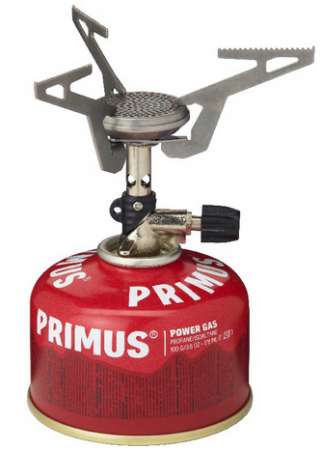
\includegraphics[width=2.5cm]{images/kocher-gas.png}
					\end{column}
				\end{columns}
			\end{frame}
				
			\begin{frame}{Outdoor-Küche: Kocher (2/4)}
				\begin{columns}[c]
					\begin{column}{0.69\textwidth}
						\textbf{Spirituskocher:}
						\begin{itemize}
							\item Becher für Spiritus
							\item Gestell für Topf
							\item[\sarrow] Simpler Aufbau, keine Kartusche, Spiritus überall verfügbar, Vorsicht bei Benutzung
						\end{itemize}
					\end{column}
					\begin{column}{0.29\textwidth}
						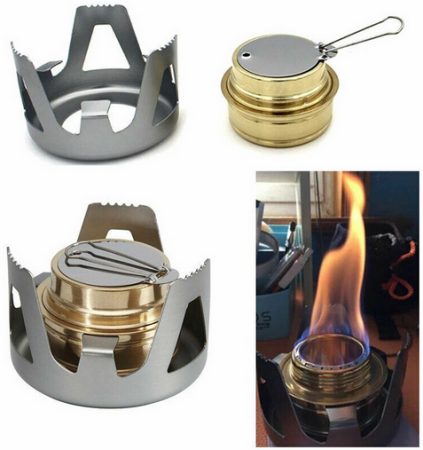
\includegraphics[width=3cm]{images/kocher-spiritus.png}
					\end{column}
				\end{columns}
			\end{frame}
		
			\begin{frame}{Outdoor-Küche: Kocher (3/4)}
				\begin{columns}[c]
					\begin{column}{0.62\textwidth}
						\textbf{Benzinkocher / Mehrstoffkocher:}
						\begin{itemize}
							\item Drucktank für Benzin (alternativ: Petroleum, Diesel, Kerosin)
							\item Vorheiz-Filz
							\item Brennkopf mit Halterung für Topf
							\item[\sarrow] Schwierige Handhabung, hohe Heizleistung, Brennstoff überall verfügbar
						\end{itemize}
					\end{column}
					\begin{column}{0.36\textwidth}
						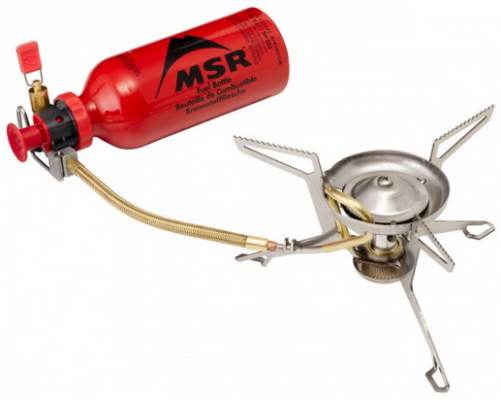
\includegraphics[width=3.85cm]{images/kocher-benzin.png}
					\end{column}
				\end{columns}
			\end{frame}
		
			\begin{frame}{Outdoor-Küche: Kocher (4/4)}
				\begin{columns}[c]
					\begin{column}{0.69\textwidth}
						\textbf{Hobokocher:}
						\begin{itemize}
							\item Kleiner Holzofen
							\item Ineinander gesteckte Bleche
							\item[\sarrow] Kleines Packmaß, Brennstoff Verfügbarkeit prüfen, ggf. illegal (z.B. in NSGs) 
						\end{itemize}
					\end{column}
					\begin{column}{0.29\textwidth}
						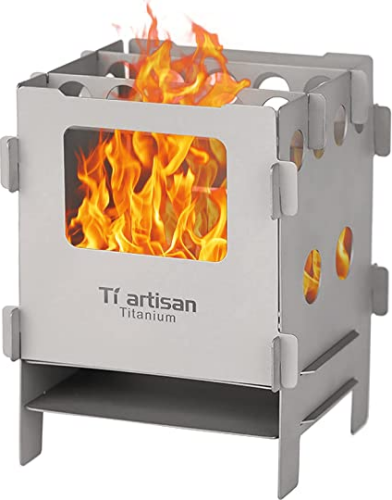
\includegraphics[width=2.35cm]{images/kocher-hobo.png}
					\end{column}
				\end{columns}
			\end{frame}
			
			\begin{frame}{Outdoor-Essen: Frühstück}
				\begin{itemize}
					\item Müsli / Porridge
					\item Rührei aus Eipulver und Wasser
					\item[\sarrow] Gerne warm, viele Kohlenhydrate \& Proteine, mäßig viel Fett, wenig/kein Zucker
				\end{itemize}\pause
				\tipp[Was manche gerne machen]{Aufstehen, eine Stunde wandern und erst dann Frühstücken}\\\pause
				\tipp[Was ich gerne mache]{Instant-Kaffeepulver mitnehmen ;)}
			\end{frame}
			
			\begin{frame}{Outdoor-Essen: Snacks}
				\begin{itemize}
					\item Müsli- oder Sportriegel (\textrightarrow\ möglichst wenig Zucker!)
					\item Nüsse
					\item Trockenfrüchte
					\item Kekse, Cracker, Knäckebrot
				\end{itemize}
			\end{frame}
			
			\begin{frame}{Outdoor-Essen: Hauptmahlzeit}
				\begin{itemize}
					\item Warme \& leckere Mahlzeit
					\item Idealerweise: Getrocknetes Essen, heißt Wasser drauf, ziehen lassen, fertig\pause
					\item Fertigprodukte:
					\begin{itemize}
						\item Sea To Summit, Trek'n Eat, ...
						\item Teuer + viel Müll
					\end{itemize}\pause
					\item Selbst mischen:
					\begin{itemize}
						\item Nudeln, Linsen, Reis, Cousous, Bulgur, Quinoa, getr. Tofu, Haferflocken
						\item Getrocknetes Gemüse, Röstzwiebeln, Samen, Kerne
						\item Eine Tüte Fertiggericht-, Suppen- oder Saucenpulver
						\item Kleines Fläschchen Öl separat mitnehmen
					\end{itemize}
					\item Nachtisch hebt die Stimmung (und liefert Kalorien)
				\end{itemize}
			\end{frame}
			
			\begin{frame}{Outdoor-Essen: Hinweise}
				\begin{itemize}
					\item Kalorienverbrauch x1,5 bis x2 ($>$ 2500-3000 / Tag)
					\begin{itemize}
						\item Fertig-Gerichte: 500 - 700 kcal
						\item Eigene Mischung: ca. 300-350 kcal / 100g
						\item Gewichtsabnahme bei längeren Wanderungen wahrscheinlich
					\end{itemize}
					\item Gerade bei längeren Touren: Es muss schmecken!
				\end{itemize}
			\end{frame}
			
			\begin{frame}{Hygiene}
				\textbf{Must have:}
				\begin{itemize}
					\item Waschlappen, Handtuch (Mikrofaser)
					\item Outdoor-Seife (einigermaßen biologisch abbaubar)
					\item Zahnputzsachen
					\item Toilettenpapier, Desinfektionsmittel
					\item Erste-Hilfe-Set
				\end{itemize}\pause
				\textbf{Optional:}
				\begin{itemize}
					\item Deo
					\item Schlafsack Inlett
				\end{itemize}\pause
				\textbf{Überbewertet (IMHO):}
				\begin{itemize}
					\item Parfum, Schmuck, Schminke o.O
					\item Schampoo, Duschgel
				\end{itemize}
			\end{frame}
			
			\begin{frame}{Werkzeuge}
				\begin{itemize}
					\item Kompass
					\item Taschenmesser, Multitool, Axt
					\item Taschenlampe, Stirnlampe
					\item Feuerzeug (besser: Feuerstahl)
				\end{itemize}
			\end{frame}
			
			\begin{frame}{Kleidung: Materialien}
				\begin{itemize}
					\item Baumwolle (\textrightarrow\ \textit{cotton kills}), Viskose, Lyocell
					\item Wolle (Schaf, Merino, Alpaka, etc.)
					\item Polyesther, Polypropylen
					\item Nylon
					\item Membrane (GoreTex, H2NO, Drilite, etc.)
				\end{itemize}
			\end{frame}
			
			\begin{frame}{Kleidung: Kopf, Hals, Hände}
				\begin{itemize}
					\item Mütze
					\item Hut
					\item Handschuhe
					\item Schal, Multifunktionstuch
				\end{itemize}
			\end{frame}
			
			\begin{frame}{Kleidung: Oberkörper}
				\begin{itemize}
					\item Top, T-Shirt, Langarmshirt, Sport-Shirts
					\item Jacke: Softshell, Hardshell, Regenjacke
					\item Poncho
				\end{itemize}\pause
				\tipp[Hinweis 1]{Regenjacken sind i.d.R. auch winddicht.}\\\pause
				\tipp[Hinweis 2]{Regenjacken bleiben nicht wasserdicht!}
			\end{frame}
			
			\begin{frame}{Kleidung: Hüftregion}
				\begin{itemize}
					\item Must have: Unterwäsche
					\item Optional: Funktionsunterwäsche
					\item Hauptsache bequem
				\end{itemize}
			\end{frame}
			
			\begin{frame}{Kleidung: Beine}
				\begin{itemize}
					\item Soft- \& Hardshell Hosen
					\item Regenhosen
					\item Normale Hosen, Cargopants, Leggins, etc.
				\end{itemize}
			\end{frame}
			
			\begin{frame}{Kleidung: Füße}
				\begin{itemize}
					\item Wandershuhe / -stiefel
					\item Wandersocken
				\end{itemize}\pause
				\tipp{Zwei-Socken-Prinzip gegen Blasen: Normale Socken und darüber Wandersocken.}
			\end{frame}
			
			\begin{frame}{Kleidung}
				\textbf{Must have:}
				\begin{itemize}
					\item Bequeme Kleidung
					\item An Witterung, Temperatur, Umgebung, Dauer, Belastung angepasst
					\item Immer trockene Wechselkleidung!
					\item Gute Wanderschuhe
					\item Socken-Strategie, die keine Blasen verursacht
				\end{itemize}\pause
				\textbf{Optional:}
				\begin{itemize}
					\item Auf Wandern angepasste Kleidung
				\end{itemize}\pause
				\textbf{Überbewertet (IMHO):}
				\begin{itemize}
					\item Super-duper Funktionskleidung
					\item Gewisse Marken (z.B. Icebreaker, Fjällräven, Arc'teryx)
				\end{itemize}
			\end{frame}
			
			\begin{frame}{Wanderstöcke}
				\begin{columns}[c]
					\begin{column}{0.69\textwidth}
						\begin{itemize}
							\item[$+$] Mehr Stabilität \& Trittsicherheit
							\item[$+$] Gewichtsverlagerung
							\item[$+$] Weniger anstrengend
							\item[$+$] Geringere Kniebelastung
							\item[$+$] Hilfreich beim Furten
							\item[$+$] Gestände beim Tarp\pause
							\item[$-$] Hände nicht mehr frei
							\item[$-$] Falsche Sicherheit
							\item[$-$] Schäden an Weg und Natur
						\end{itemize}
					\end{column}
					\begin{column}{0.29\textwidth}
						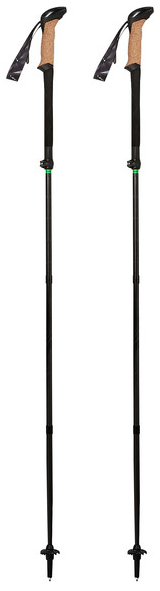
\includegraphics[width=1.25cm]{images/hiking-sticks.png}
					\end{column}
				\end{columns}
			\end{frame}
		
		\subsection{Karten}
			
			\begin{frame}{Arten}
				\begin{minipage}{0.59\textwidth}
					\textbf{Relevante Rubriken:}
					\begin{itemize}
						\item<1-> Stadtpläne, Straßenkarten
						\item<1-> Fahrradkarten
						\item<1-> Gewässerkarten
						\item<2-> Luftbildkarten
						\item<3-> Thematische Karten
						\item<4-> Wanderkarten
						\item<4-> Topografische Karten
					\end{itemize}
				\end{minipage}
				\begin{minipage}{0.39\textwidth}
					\onslide<1->{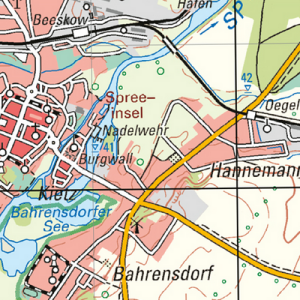
\includegraphics[height=2cm]{images/map-example-street.png}}
					\onslide<2->{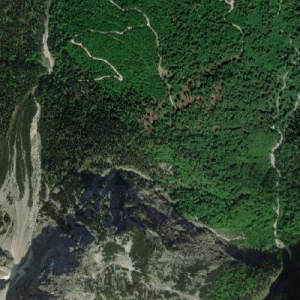
\includegraphics[height=2cm]{images/map-example-aerial.png}}\vspace{0.1cm}\\\noindent
					\onslide<3->{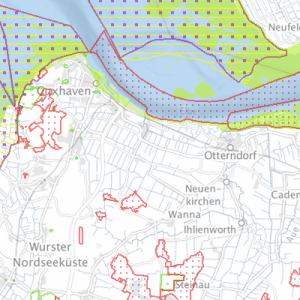
\includegraphics[height=2cm]{images/map-example-thematic.png}}
					\onslide<4->{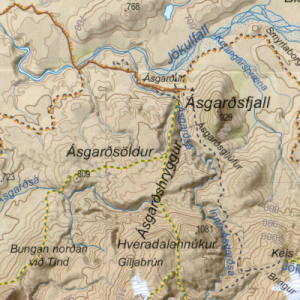
\includegraphics[height=2cm]{images/map-example-hiking.png}}
				\end{minipage}
			\end{frame}
			
			\begin{frame}{Bestandteile}
				\begin{minipage}{0.59\textwidth}
					\begin{itemize}
						\item<1-> Legende
						\item<2-> Maßstab
						\item<3-> Koordinaten
						\item<4-> Ggf. Nordpfeil
					\end{itemize}
				\end{minipage}
				\begin{minipage}{0.39\textwidth}
					\onslide<1->{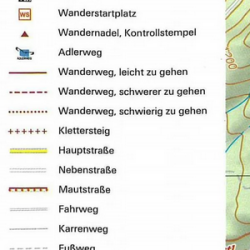
\includegraphics[height=2cm]{images/map-legend.png}}
					\onslide<2->{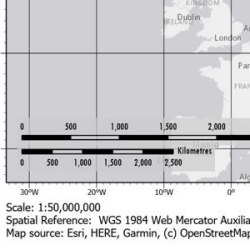
\includegraphics[height=2cm]{images/map-scale.png}}\vspace{0.1cm}\\\noindent
					\onslide<3->{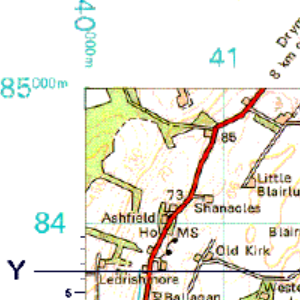
\includegraphics[height=2cm]{images/map-coordinates.png}}
					\onslide<4->{
\includegraphics[height=2cm]{images/map-north-arrow.png}}
				\end{minipage}
			\end{frame}
			
			\begin{frame}{Topografische Karten lesen (1/2)}
				\begin{center}
					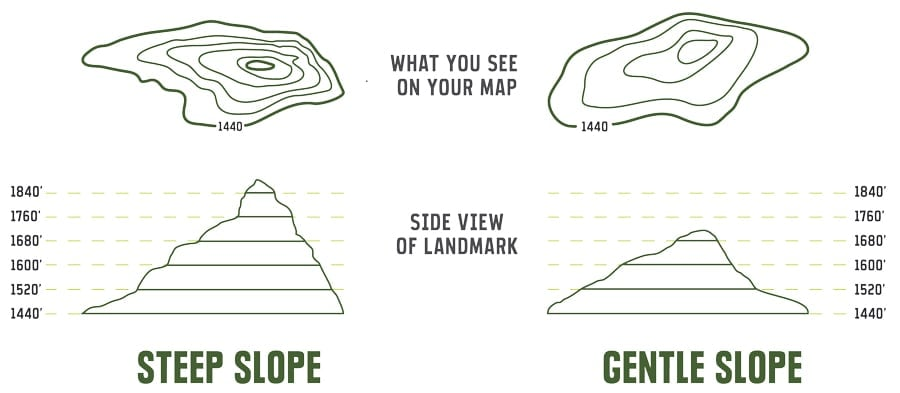
\includegraphics[width=0.8\textwidth]{images/map-topo-rei.jpg}
				\end{center}
				{\hfill\tiny Bildquelle: \href{https://www.rei.com/learn/expert-advice/topo-maps-how-to-use.html}{rei.com}}
			\end{frame}
			
			\begin{frame}{Topografische Karten lesen (2/2)}
				\begin{center}
					\begin{tikzpicture}
						[
							font=\scriptsize
						]
						\node[anchor=south west,inner sep=0] (image) at (0,0) {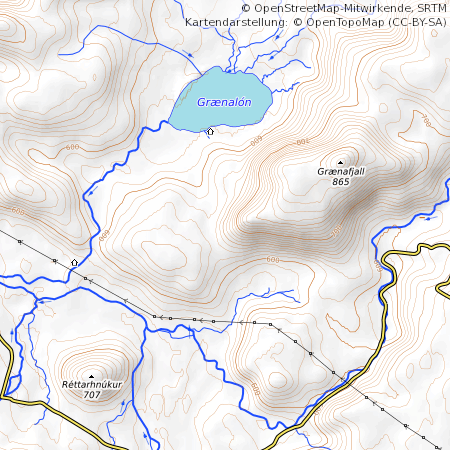
\includegraphics[height=0.75\textheight]{images/map-topo-base.png}};
						
						\begin{scope}[x={(image.south east)},y={(image.north west)}]
%							\draw[help lines,xstep=.1,ystep=.1] (0,0) grid (1,1);
%							\foreach \x in {0,1,...,9} { \node [anchor=north] at (\x/10,0) {\tiny 0.\x}; }
%							\foreach \y in {0,1,...,9} { \node [anchor=east] at (0,\y/10) {\tiny 0.\y}; }
							
							\only<1>{
								\node[red] (gipfel) at (0.5, 0.05) {\contour{white}{Gipfel}};
								\draw[thick,red,->] (gipfel) -- (0.21,0.16);
								\draw[thick,red,->] (gipfel) -- (0.37,0.43);
							}
							
							\only<2>{
								\node[red] (valley) at (0.3, 0.05) {\contour{white}{Tal}};
								\draw[thick,red,->] (valley) -- (0.22,0.46);
								\draw[thick,red,->] (valley) -- (0.5,0.27);
								\node[red] (saddle) at (0.75, 0.05) {\contour{white}{Sattel}};
								\draw[thick,red,->] (saddle) -- (0.48,0.45);
								\draw[thick,red,->] (saddle) -- (0.7,0.31);
							}
							
							\only<3>{
								\node[red] (flat) at (0.5, 0.05) {\contour{white}{Flache Ebene}};
								\draw[thick,red,->] (flat) -- (0.19,0.31);
								\draw[thick,red,->] (flat) -- (0.37,0.65);
							}
							
							\only<4>{
								\node[red] (gentle) at (0.5, 0.05) {\contour{white}{Seichter Anstieg}};
								\draw[thick,red,->] (gentle) -- (0.175,0.48);
								\draw[thick,red,->] (gentle) -- (0.95,0.27);
							}
							
							\only<5>{
								\node[red] (gentle) at (0.38, 0.05) {\contour{white}{Steiler Anstieg}};
								\draw[thick,red,->] (gentle) -- (0.42,0.32);
								\node[red] (cliff) at (0.72, 0.05) {\contour{white}{Klippe}};
								\draw[thick,red,->] (cliff) -- (0.64,0.44);
							}
							
							\only<6>{
								\node[red] (view) at (0.5, 0.05) {\contour{white}{Geile Aussicht}};
								\draw[thick,red,->] (view) -- (0.05,0.56);
								\draw[thick,red,->] (view) -- (0.56,0.51);
								\draw[thick,red,->] (view) -- (0.63,0.62);
							}
						\end{scope}
					\end{tikzpicture}
				\end{center}
			\end{frame}
		
		\subsection{Navigation}
			
			\begin{frame}{Equipment}
				\begin{minipage}{0.59\textwidth}
					\begin{itemize}
						\item<1-> Karte \& Kompass
						\begin{itemize}
							\item Kartenausrichtung
							\item Orientierung, Wegfindung
							\item Positionsbestimmung
						\end{itemize}
						\item<2-> Handy, GPS-Gerät
						\item<3-> Sonne, Mond, Sterne
						\item<3-> Uhr
						\begin{itemize}
							\item Orientierung mit Uhrzeit und Sonne
						\end{itemize}
					\end{itemize}
				\end{minipage}
				\begin{minipage}{0.39\textwidth}
					\only<1>{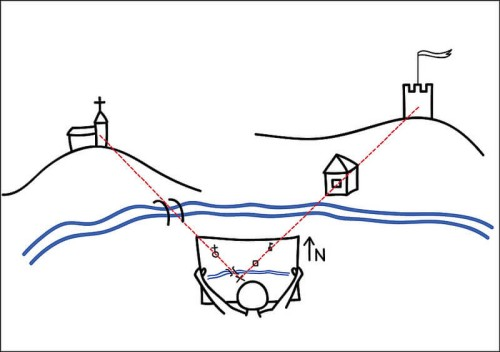
\includegraphics[width=4cm]{images/navigation-map-positioning.jpg}}
					\only<2>{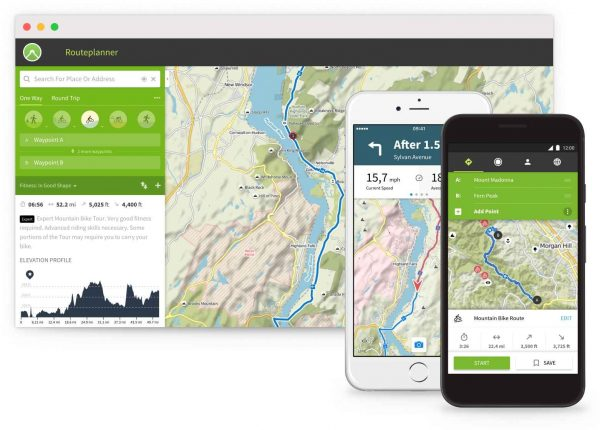
\includegraphics[width=4cm]{images/navigation-app.jpg}}
					\only<3>{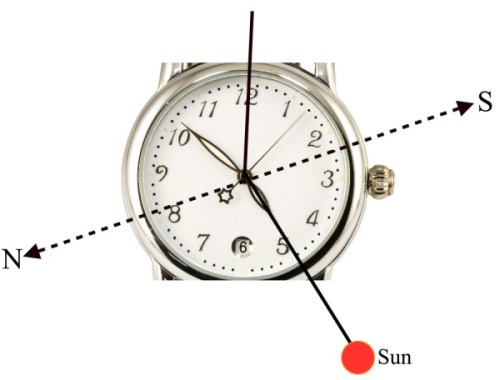
\includegraphics[width=4cm]{images/navigation-clock-sun.jpg}}
				\end{minipage}
			\end{frame}
	
	\section{Tourenplanung}
		
		\begin{frame}[t]{Inhalt}
			\tableofcontents[currentsection,hideothersubsections]
		\end{frame}
	
		\subsection{Tagestouren}
			
			\begin{frame}{}
			\end{frame}
			
		\subsection{Mehrtägige Touren}
			
			\begin{frame}{}
			\end{frame}
		
		\subsection{Mehrwöchige Touren}
			
			\begin{frame}{}
			\end{frame}
		
		\subsection{Noch längere Touren}
			
			\begin{frame}{}
			\end{frame}
	
	\section{Richtiges Verhalten}
		
		\begin{frame}[t]{Inhalt}
			\tableofcontents[currentsection,hideothersubsections]
		\end{frame}
		
		\subsection{Verhaltensweisen: Do's \& Don'ts}
			
			\begin{frame}{}
			\end{frame}
			
		\subsection{Sicherheit}
			
			\begin{frame}{}
			\end{frame}
	
	\section{Rechtliches, Tipps \& Tricks}
		
		\begin{frame}[t]{Inhalt}
			\tableofcontents[currentsection,hideothersubsections]
		\end{frame}
	
		\subsection{Rechtliche Lage}
			
			\begin{frame}{}
			\end{frame}
		
		\subsection{Tipps \& Tricks}
\end{document}